\subsection{Models}
    \subsubsection{Decision Tree Classifier}
        Constructs a decision tree to classify data based on features\\
        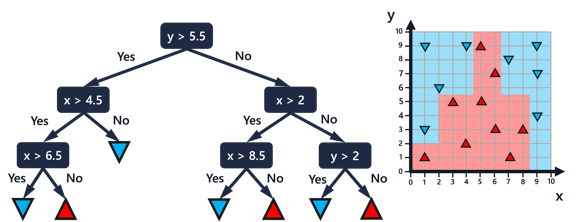
\includegraphics[width = \linewidth]{src/8_ml/images/decision_tree.png}
        \lstinputlisting{src/8_ml/code/decision_tree_classifier.py}

    \subsubsection{Linear}
        {\centering \underline{\textbf{Regression}} \par}
        Constructs a linear model $y = \beta_0 + \sum_{i = 0}^n \beta_i x_i$ so that the loss function is minimized
        {\centering 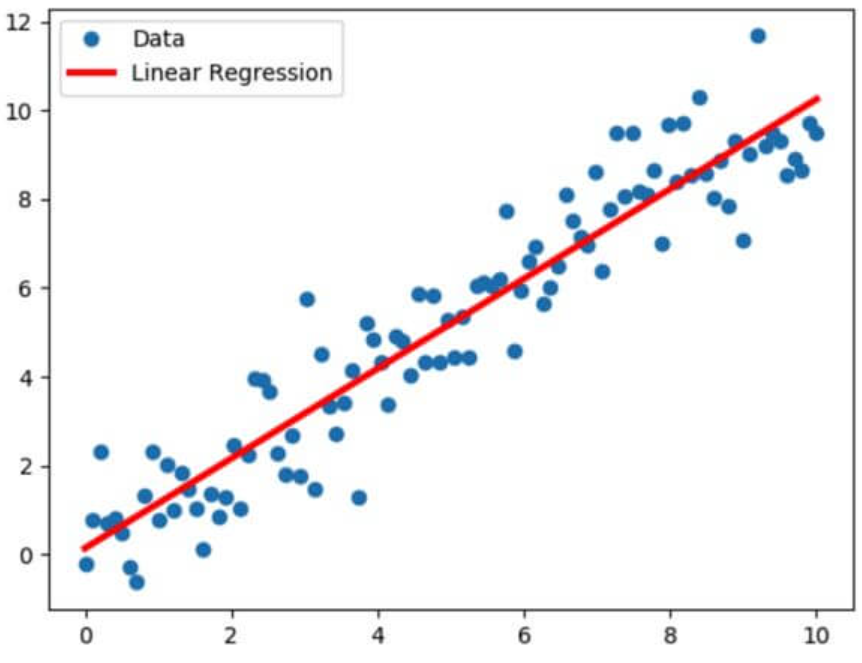
\includegraphics[width = 0.8\linewidth]{src/8_ml/images/linear_regression.png} \par}
        \lstinputlisting{src/8_ml/code/linear_regression.py}
        
        {\centering \underline{\textbf{Classification}} \par}
        {\centering 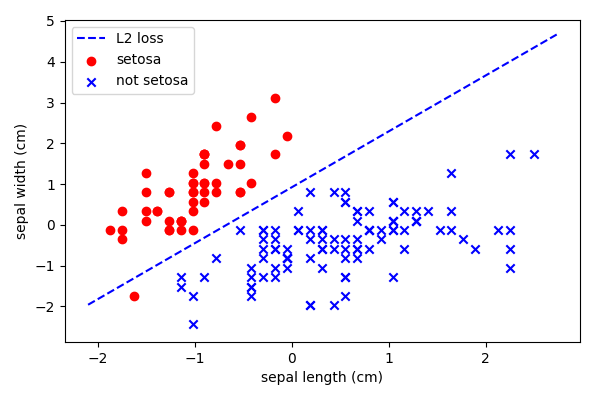
\includegraphics[width = 0.8\linewidth]{src/8_ml/images/linear_classifier.png} \par}

    \subsubsection{Neural Network}
        Constructs layers of neurons, where the output of each neuron is made non-linear through an activation function (Sigmoid, Relu, Tanh)\\
        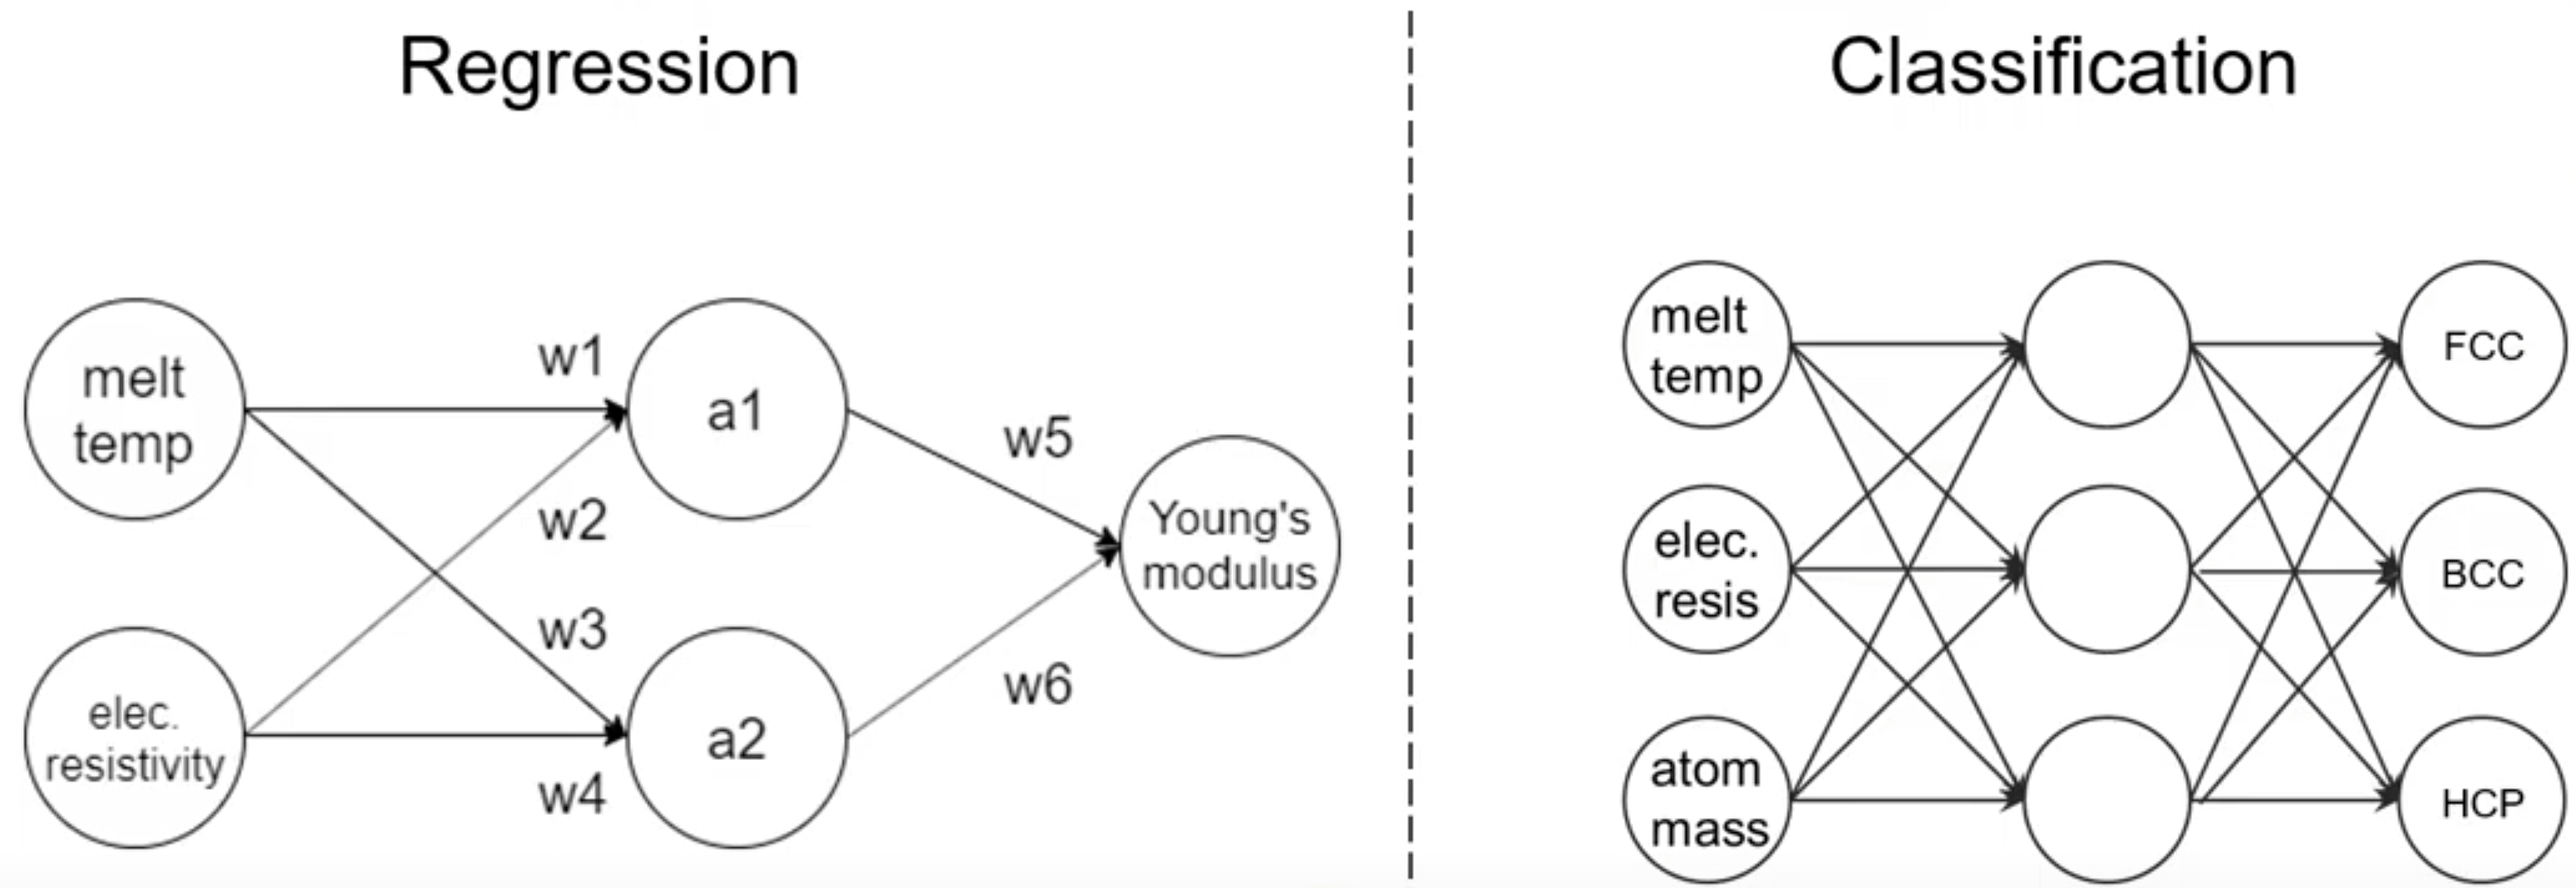
\includegraphics[width = \linewidth]{src/8_ml/images/neural_network_regression_vs_classifier.png}
        
        {\centering \underline{\textbf{Regression}} \par}
        Usually no activation function in output layer\\
        \lstinputlisting{src/8_ml/code/mlpregressor.py}
        
        {\centering \underline{\textbf{Classification}} \par}
        Usually Sigmoid in output layer\\
        \lstinputlisting{src/8_ml/code/mlpclassifier.py}
        
        {\centering \underline{\textbf{Convolutional Neural Network}} \par}
    	Softmax can be used in output layer\\
        Image processing, process to reduce data\\
        Example using Joint Matrix (Faltungsmatrix):
        {\centering 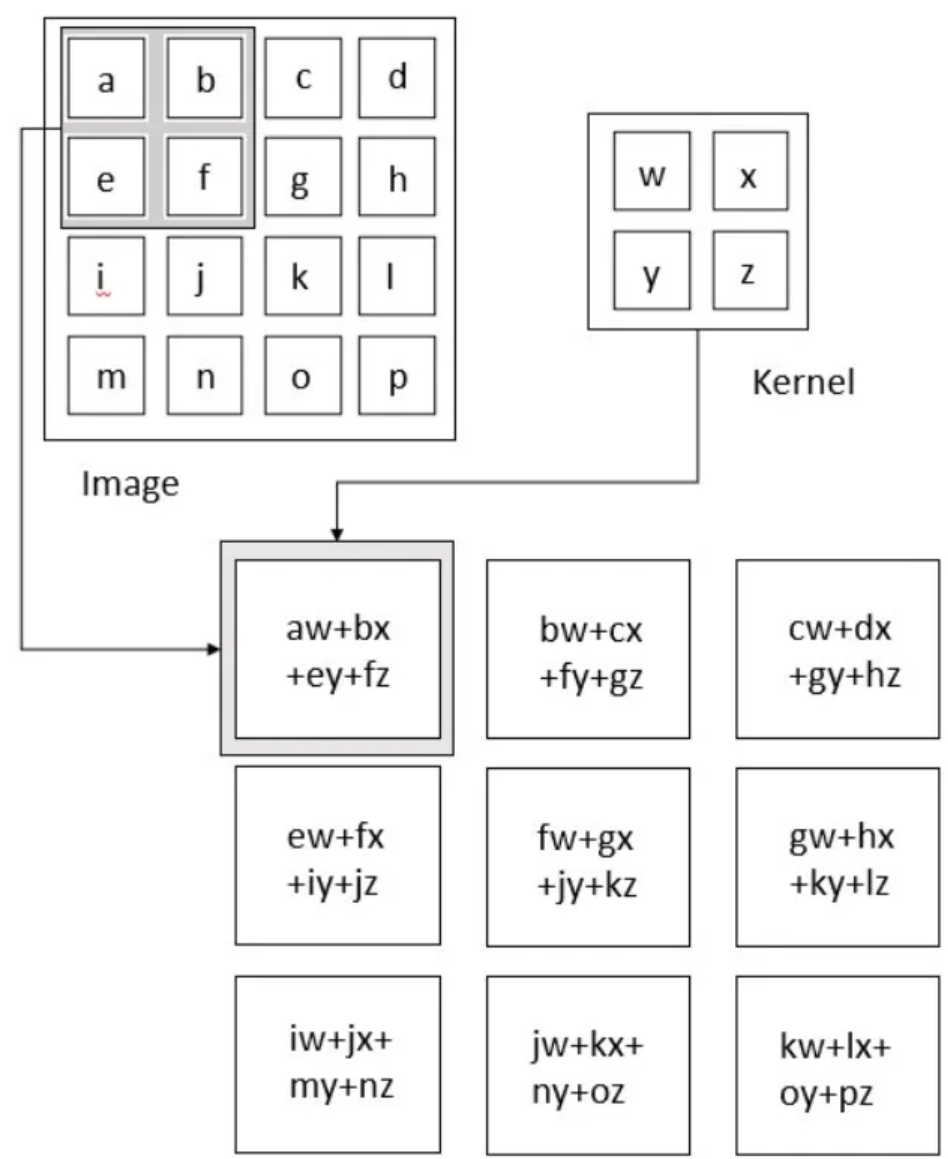
\includegraphics[width = 0.8\linewidth]{src/8_ml/images/convolutional.png} \par}
        One can also choose the max matrix. For the first field in the example this would yield the output: $\text{max}(a, b, e, f)$